\documentclass[10pt]{article}

\usepackage{amsthm}
\usepackage{amsmath}
\usepackage{amssymb}
\usepackage{mathtools}
\usepackage{graphicx}
\usepackage[colorinlistoftodos]{todonotes}
\usepackage{url}
\usepackage{xcolor}

\usepackage{pgfplots}

\usepackage[left = 1cm, top = 1cm, bottom = 2cm, right = 1cm, nohead, nofoot]{geometry}

\pgfplotsset{width=19cm, compat=1.3}

\newcommand{\C}{\mathbb{C}}  % Complex
\newcommand{\R}{\mathbb{R}}  % Real
\newcommand{\Z}{\mathbb{Z}}  % Integers
\newcommand{\N}{\mathbb{N}}  % Naturals

\newcommand{\A}{\mathbb{A}}
\newcommand{\K}{\mathbb{K}}

\title{$\A$dvanced $\C$alculus}
\author{$\C$ason $\K$onzer}
\date{October 20, 2021}



\begin{document}
\maketitle

\newpage

\section{\underline{}}
\label{sec: Problem 1}
\noindent
Find the general solution of the ODE $ y'' + 9y = r(t) $, where $ \displaystyle r(t) = \frac{\pi}{4} |\sin{t}| $ for $ 0 < t < 2\pi $ and $ r(t + 2\pi) = r(t) $. \\
\vspace{2.5mm}
\hrule 

\vspace{7.5mm}

\noindent
\textbf{First} solve the homogeneous solution $ y_h \ | \ y'' + 9y = 0 $. \\

\begin{itemize}
    \item $ \displaystyle h^2 + 9 = 0 \ ; \ h^2 = -9 \ ; \ h = \sqrt{-9} \ ; \ h = \pm 3i $. \\
    \item $ \displaystyle y_h = c_1 cos(3t) + c_2 sin(3t) $. \\
\end{itemize}

\noindent
\textbf{Second} solve the forcing function $ \displaystyle r = \frac{\pi}{4} |\sin{t}| $ for $ 0 < t < 2\pi $ with period, $ p = 2\pi \ ; \ L = \pi $. \\

\begin{center}
    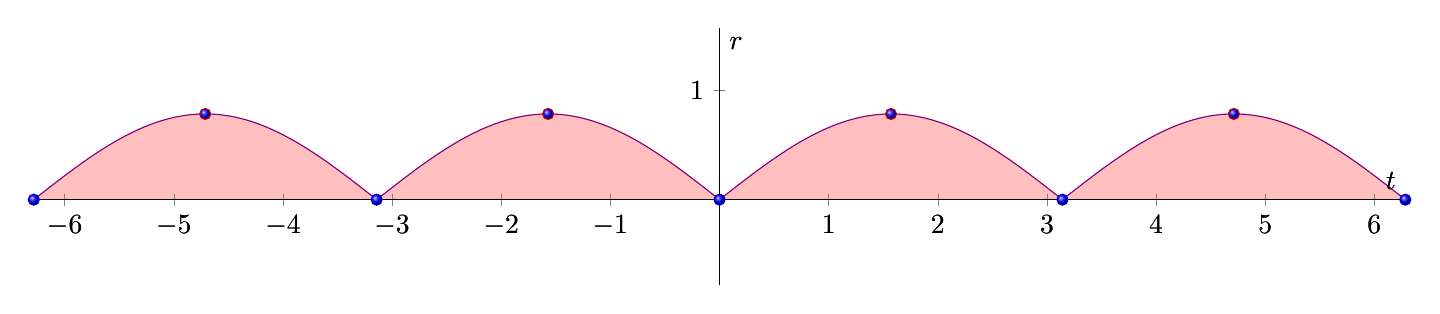
\begin{tikzpicture}
        \begin{axis}[
            xlabel = $ t $, ylabel = $ r $,
            xmin = -2*pi, xmax = 2*pi,
            ymin = -pi/4 , ymax = pi/2,
            try min ticks =  2,
            axis equal image = true,
            axis x line=center,
            axis y line=center,
            axis line style = -,
        ]
            \addplot[
                no marks,
                color = pink,
                fill
            ]
                expression[
                    domain = -4*pi : 4*pi,
                    samples = 710
                ]
                    {(pi/4)*abs(sin(deg(x)))}
            ;
            \addplot[
                no marks,
                color = violet,
            ]
                expression[
                    domain = -4*pi : 4*pi,
                    samples = 710
                ]
                    {(pi/4)*abs(sin(deg(x)))}
            ;
        \end{axis}
        \begin{axis}[
            xlabel = $ t $, ylabel = $ r $,
            xmin = -2*pi, xmax = 2*pi,
            ymin = -pi/4 , ymax = pi/2,
            try min ticks =  2,
            axis equal image = true,
            axis x line=center,
            axis y line=center,
            axis line style = -,
        ]
            \addplot[
                only marks,
                mark = ball,
                color = violet,
                scatter
            ]
                coordinates{
                    (-2*pi, 0) (-pi, 0) (0,0) (pi, 0) (2*pi,0)
                    (-5*pi/2, pi/4) (-3*pi/2, pi/4) (-pi/2, pi/4) (pi/2, pi/4) (3*pi/2, pi/4) (5*pi/2, pi/4)
                }
            ; 
        \end{axis}
    \end{tikzpicture} \\
\end{center}

\begin{itemize}
    \item Notice r is even thus the $ Euler $ coefficent $ b_n = 0 $. Solve for $ a_0 $ and $ a_n $. \\
    \item $ \displaystyle a_0 = \frac{1}{\pi}  \int_{0}^{\pi} \frac{\pi}{4} |\sin{t}| \,dt $ ; note $ sin(t) $ is positive for all $ t \ | \ 0 < t < \pi $. \\
    \subitem $ \displaystyle a_0 = \frac{1}{4} [- cos(t) \Big|_{0}^{\pi}] = \frac{- cos(\pi) + cos(0)}{4} = \frac{1 + 1}{4} = \frac{1}{2} $. 
    \item $ \displaystyle a_n = \frac{2}{\pi}  \int_{0}^{\pi} \frac{\pi}{4} |\sin{t}| \cos(\frac{n\pi t}{\pi}) \,dt = \frac{1}{2}  \int_{0}^{\pi} \sin{t} \cos(nt) \,dt $. $ \dagger $ Invoke Mathematica $ \dots $ \\
    \subitem $ \displaystyle a_n = \frac{1}{2} [\frac{nsin(t)sin(nt) + cos(t)cos(nt)}{n^2 - 1} \Big|_{0}^{\pi}] $.
    \subitem $ \displaystyle a_n = \frac{1}{2} [\frac{(nsin(\pi)sin(n\pi) + cos(\pi)cos(n\pi)) - (nsin(0)sin(0) + cos(0)cos(0))}{n^2 - 1}] $. \\ 
    \subitem $ \displaystyle a_n = \frac{1}{2} [\frac{- cos(n\pi) - 1}{n^2 - 1}] $ ; note $ cos(n\pi) = 1 \ | \ n \ even \ ; \ cos(n\pi) = -1 \ | \ n \ odd $.
    \subitem $ \displaystyle a_n = \frac{1}{2} [\frac{- 1 - 1}{n^2 - 1}] = \frac{- 1}{n^2 - 1} \ | \ n \ even $. 
    \item $ \displaystyle r = a_0 + \sum_{n = 1}^{\infty} (a_n \cos(nt) + b_n \sin (nt)) $ \\
    \subitem $ \displaystyle r = \frac{1}{2} - \sum_{n = 2 \ | n \ even}^{\infty} \frac{1}{n^2 - 1} \cos(nt) $.
    \subitem $ \displaystyle r = \frac{1}{2} - \frac{1}{2^2 - 1} \cos(2t)  - \frac{1}{4^2 - 1} \cos(4t)  - \frac{1}{6^2 - 1} \cos(6t) - \dots $.
    \subitem $ \displaystyle r = \frac{1}{2} - \frac{1}{3} \cos(2t)  - \frac{1}{15} \cos(4t)  - \frac{1}{35} \cos(6t) - \frac{1}{63} \cos(8t) - \dots $. \\
\end{itemize} 
\newpage

\noindent
\textbf{Third} solve the particular solution $ y_p \ | \ y'' + 9y = r(t) $. \\

\begin{itemize}
    \item $ \displaystyle y = A_0 + A \cos(nt) \ ; \ y' = -An \sin(nt) \ ; \ y'' = -An^2 \cos(nt) $. \\
    \item $ \displaystyle -An^2 \cos(nt) + 9A \cos(nt) + 9A_0 = \frac{1}{2} - \frac{1}{n^2 - 1} \cos(nt) $. \\
    \subitem $ \displaystyle A_0 = \frac{1}{18} $.
    \subitem $ \displaystyle A(9 - n^2) = \frac{-1}{n^2 - 1} \ ; \ A = \frac{-1}{(n^2 - 1)(9 - n^2)} $.
    \item $ \displaystyle y_p = A_0 + \sum_{n = 2 \ | n \ even}^{\infty} Acos(nt) =  \frac{1}{18} - \sum_{n = 2 \ | n \ even}^{\infty} \frac{cos(nt)}{(n^2 - 1)(9 - n^2)} $ . \\
    \subitem $ \displaystyle y_p = \frac{1}{18} - \frac{cos(2t)}{(2^2 - 1)(9 - 2^2)} - \frac{cos(4t)}{(4^2 - 1)(9 - 4^2)} - \frac{cos(6t)}{(n^2 - 1)(9 - 6^2)} \dots $
    \subitem $ \displaystyle y_p = \frac{1}{18} - \frac{cos(2t)}{(3)(5)} - \frac{cos(4t)}{(15)(-7)} - \frac{cos(6t)}{(35)(-27)} - \frac{cos(8t)}{(63)(-54)} \dots $
    \subitem $ \displaystyle y_p = \frac{1}{18} - \frac{cos(2t)}{15} + \frac{cos(4t)}{105} + \frac{cos(6t)}{945} + \frac{cos(8t)}{3402} \dots $ \\
\end{itemize}

\noindent
\textbf{Last} combine to form the general solution $ y = y_h + y_p $. \\

\begin{itemize}
    \item $ \displaystyle y = c_1 cos(3t) + c_2 sin(3t) + \frac{1}{18} - \sum_{n = 2 \ | n \ even}^{\infty} \frac{cos(nt)}{(n^2 - 1)(9 - n^2)} $.
\end{itemize}


\newpage


\section{\underline{}}
\label{sec: Problem 2}
\noindent
For $ f(x) = x $ on $ -\pi < x < \pi $, find the trigonometric polynomial $ \displaystyle F(x) = A_0 + \sum_{n = 1}^N (A_n\cos(nx) + B_n\sin(nx)) $ that minimizes $ ||f-F||_2 $ on $ (-\pi, \pi) $, for $ N = 1, 3, 5 $. \\
\vspace{2.5mm}
\hrule

\vspace{7.5mm}

\noindent
\textbf{Find} the Fourier Series $ \ | \ \ p = 2\pi \ ; \ L = \pi $ \\

\begin{center}
    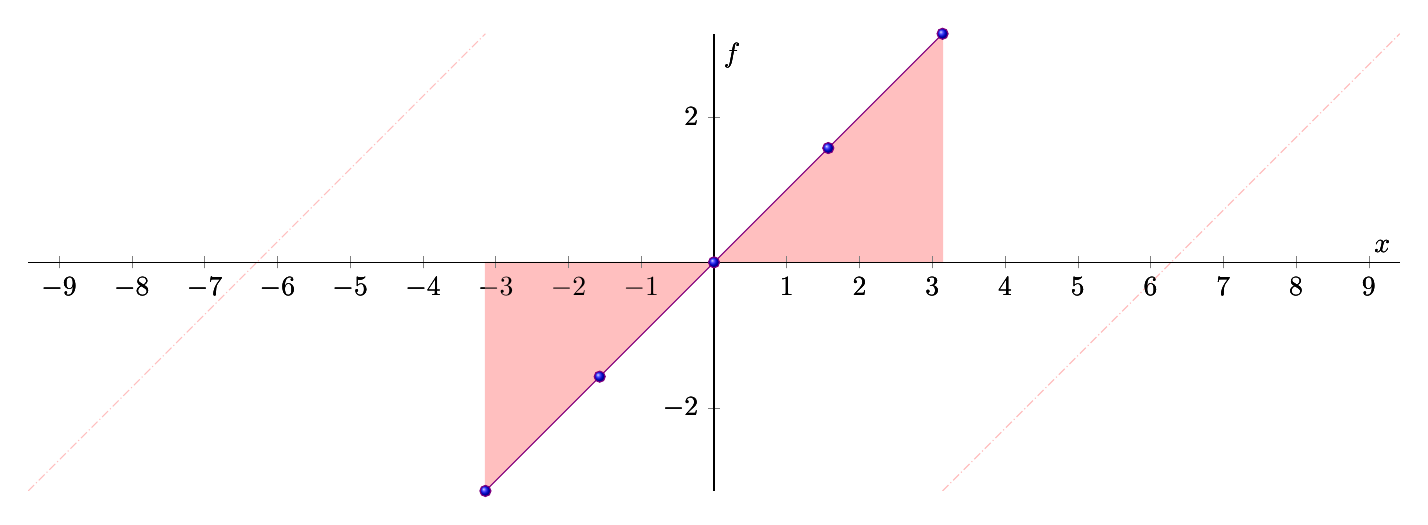
\begin{tikzpicture}
        \begin{axis}[
            xlabel = $ x $, ylabel = $ f $,
            xmin = -3*pi, xmax = 3*pi,
            ymin = -pi , ymax = pi,
            try min ticks =  2,
            axis equal image = true,
            axis x line=center,
            axis y line=center,
            axis line style = -,
            style = densely dashdotted 
        ]
            \addplot[
                no marks,
                color = pink
            ]
                expression[
                    domain = -3*pi : -pi,
                    samples = 3
                ]
                    {x + 2*pi}
            ;
            \addplot[
                no marks,
                color = pink
            ]
                expression[
                    domain = pi : 3*pi,
                    samples = 3
                ]
                    {x - 2*pi}
            ;
        \end{axis}
        \begin{axis}[
            xlabel = $ x $, ylabel = $ f $,
            xmin = -3*pi, xmax = 3*pi,
            ymin = -pi , ymax = pi,
            try min ticks =  2,
            axis equal image = true,
            axis x line=center,
            axis y line=center,
            axis line style = -,
        ]
            \addplot[
                no marks,
                color = pink,
                fill
            ]
                expression[
                    domain = -pi : pi,
                    samples = 3
                ]
                    {x}
                \closedcycle
            ;
        \end{axis}
        \begin{axis}[
            xlabel = $ x $, ylabel = $ f $,
            xmin = -3*pi, xmax = 3*pi,
            ymin = -pi , ymax = pi,
            try min ticks =  2,
            axis equal image = true,
            axis x line=center,
            axis y line=center,
            axis line style = -,
        ]
            \addplot[
                mark = ball,
                color = violet
            ]
                expression[
                    domain = -pi : pi,
                    samples = 5
                ]
                    {x}
            ;
        \end{axis}
    \end{tikzpicture} \\
\end{center}

\begin{itemize}
    \item Notice r is odd thus the $ Euler $ coefficents $ a_0, a_n = 0 $. Solve for $ b_n $. \\
    \item $ \displaystyle b_n = \frac{2}{\pi}  \int_{0}^{\pi}  x \sin(\frac{n\pi x}{\pi}) \,dx = \frac{2}{\pi}  \int_{0}^{\pi} x \sin(nx) \,dx $. $ \dagger $ Invoke Mathematica $ \dots $ \\
    \subitem $ \displaystyle b_n = \frac{2}{\pi} [\frac{sin(nx) - nx cos(nx)}{n^2} \Big|_{0}^{\pi}] = \frac{2}{\pi} [\frac{(sin(n \pi) - n \pi cos(n \pi)) - (sin(0) - 0)}{n^2}] $.
    \subitem $ \displaystyle b_n = \frac{2}{\pi} [\frac{- n \pi cos(n \pi)}{n^2}]  = \frac{- 2 cos(n \pi)}{n} $ ; note $ cos(n\pi) = 1 \ | \ n \ even \ ; \ cos(n\pi) = -1 \ | \ n \ odd $.
    \subitem $ \displaystyle b_n = B_n = -\frac{2}{n} \ | \ n \ even \ ; \ \frac{2}{n} \ | \ n \ odd $.
    \item $ \displaystyle f = a_0 + \sum_{n = 1}^{\infty} (a_n \cos(nx) + b_n \sin (nx)) = F = A_0 + \sum_{n = 1}^{\infty} (A_n\cos(nx) + B_n\sin(nx)) $. \\
    \subitem $ \displaystyle F_N = \sum_{n = 1 \ | \ n \ odd}^N + \frac{2}{n} \sin(nx) - \sum_{n = 2 \ | \ n \ even}^N + \frac{2}{n} \sin(nx) $.
    \subitem $ \displaystyle F_{N = 1} = 2 \sin(x) $.
    \subitem $ \displaystyle F_{N = 3} = 2 \sin(x) - \sin(2x) + \frac{2}{3} \sin(3x) $.
    \subitem $ \displaystyle F_{N = 5} = 2 \sin(x) - \sin(2x) + \frac{2}{3} \sin(3x) - \frac{1}{2} \sin(4x) + \frac{2}{5} \sin(5x) $.    
\end{itemize} 


\newpage


\section{\underline{}}
\label{sec: Problem 3}
\noindent
Refer to problem 2 to complete problem 3. Use software to compute $ ||f-F||_2 $ for $ N = 1, 3, 5 $. Then use the fact that $ \displaystyle \sum_{n = 1}^\infty \frac{1}{n^2} = \frac{\pi^2}{6} $ to show $ \displaystyle \lim_{N\to\infty}(||f-F||_2)^2 = \lim_{N\to\infty}E^*(N) = 0 $. \\
\vspace{2.5mm}
\hrule

\vspace{7.5mm}

\noindent
\textbf{Recall} our solutions from 2. \textbf{Recall} $ \displaystyle ||f-F||_2 = \sqrt{\int_{R} (f - F)^2 \,dx} $. \\

\begin{itemize} 
    \item $ \displaystyle f = x \ | \ -\pi < x < \pi \ ; \ F_N = \sum_{n = 1 \ | \ n \ odd}^N + \frac{2}{n} \sin(nx) - \sum_{n = 2 \ | \ n \ even}^N + \frac{2}{n} \sin(nx) $. \\
    \item $ \displaystyle F_{N = 1} = 2 \sin(x) $. \\
    \subitem $ \displaystyle f - F_{N = 1}  = x - 2 \sin(x) $
    \subitem $ \displaystyle ||f-F_{N = 1}||_2  = \sqrt{\int_{-\pi }^{\pi } (x - 2 \sin(x))^2 \, dx} = 2.84684$
    \item $ \displaystyle F_{N = 3} = 2 \sin(x) - \sin(2x) + \frac{2}{3} \sin(3x) $. \\
    \subitem $ \displaystyle f - F_{N = 3}  = x - 2 \sin(x) + \sin(2x) - \frac{2}{3} \sin(3x) $
    \subitem $ \displaystyle ||f-F_{N = 3}||_2  = \sqrt{\int_{-\pi }^{\pi } (x - 2 \sin(x) + \sin(2x) - \frac{2}{3} \sin(3x))^2 \, dx} = 1.88855 $
    \item $ \displaystyle F_{N = 5} = 2 \sin(x) - \sin(2x) + \frac{2}{3} \sin(3x) - \frac{1}{2} \sin(4x) + \frac{2}{5} \sin(5x) $. \\
    \subitem $ \displaystyle f - F_{N = 5}  = x - 2 \sin(x) + \sin(2x) - \frac{2}{3} \sin(3x) + \frac{1}{2} \sin(4x) - \frac{2}{5} \sin(5x) $
    \subitem $ \displaystyle ||f-F_{N = 5}||_2  = \sqrt{\int_{-\pi }^{\pi } (x - 2 \sin(x) + \sin(2x) - \frac{2}{3} \sin(3x) + \frac{1}{2} \sin(4x) - \frac{2}{5} \sin(5x))^2 \, dx} = 1.50949 $
\end{itemize}

\noindent
\textbf{Recall} $ \displaystyle ||f-F||_2 = E $ and as $ A_0 = a_0, \ A_n = a_n, \ B_n = b_n \ ; \ E = E^* $. \textbf{Thus} $ \displaystyle \lim_{N\to\infty}(||f-F||_2)^2 = \lim_{N\to\infty}E(N) = \lim_{N\to\infty}E^*(N) \dots $ \\

\noindent
\textbf{Find} $ \displaystyle E^* = \int_{-\pi }^{\pi } f^2 \, dx - \pi [2 a^2_0 + \sum_{n = 1}^{N} (a^2_n + b^2_n)] $. \\
\begin{itemize} 
    \item $ \displaystyle E^* = \int_{-\pi }^{\pi } f^2 \, dx - \pi \sum_{n = 1}^{N} b^2_n $. \\
    \subitem $ \displaystyle \int_{-\pi }^{\pi } f^2 \, dx = \int_{-\pi }^{\pi } x^2 \, dx = \frac{x^3}{3} \Big|_{-\pi}^{\pi} = \frac{\pi^3}{3} + \frac{\pi^3}{3} = \frac{2\pi^3}{3} $
    \subitem $ \displaystyle \pi \sum_{n = 1}^{N} b^2_n = \pi \sum_{n = 1}^{N} ((-1)^{n - 1} \frac{2}{n})^2 = \pi \sum_{n = 1}^{N} (-1)^{2(n-1)} \frac{4}{n^2} = \pi \sum_{n = 1}^{N} \frac{4}{n^2} = 4\pi \sum_{n = 1}^{N} \frac{1}{n^2} $
\end{itemize}

\noindent
\textbf{Find} $ \lim_{N\to\infty}E^*(N) $.
\begin{itemize} 
    \item $ \displaystyle \lim_{N\to\infty}E^*(N) = \int_{-\pi }^{\pi } f^2 \, dx - \pi \sum_{n = 1}^{\infty} b^2_n = \frac{2 \pi^3}{3} - 4\pi \sum_{n = 1}^{\infty} \frac{1}{n^2} = \frac{2 \pi^3}{3} - 4\pi (\frac{\pi^2}{6}) = \frac{2 \pi^3}{3} - \frac{2 \pi^3}{3} = 0 $
\end{itemize}

\end{document}

%Comments - October 20, 2021 Advanced Calculus Written Home Work #3%